
\newpage
\chapter{Data Sources and Elaboration}
\section{Data Sources}
The collection of the data has been an important phase during this work. \\
Several sources have been checked and consulted in order to find reliable and useful data for the final purpose of this thesis.\\
In this particular case the main data collection way was internet, but some important data have been provided also from SINTEF Nord.
\citation{}

\subsection{Data from SINTEF Nord}
Some of the data used during this thesis were provided from the team members of the eSushi project team at SINTEF Nord. \\
The data are about each single norwegian county and with the following details:\\

\begin{table}[ht]
\makebox[\textwidth][c]{
\resizebox{1.21\textwidth}{!}{
    \begin{tabular}{ | l | l | l | l | l |}
            \hline \textbf{Input}	&	\textbf{Content}	& \textbf{Unit}  & \textbf{Frequency}  & \textbf{Available Period} \\ \hline
\multicolumn{1}{|p{4cm}|}{\raggedright 1. Average Sea Temperature}	&	
\multicolumn{1}{p{4cm}|}{\raggedright Reported number of cages with salmon and rainbow trout.}
								& Celsius & Monthly & January 2007 - April 2014 	\\ \hline	
\end{tabular}}}
    \caption{Data provided from SINTEF Nord.}
    \label{table: SINTEF_Data} 
\end{table}



\newpage
 
\subsection{Data from Fiskeridir} 
The current website has been the main data source for this work. It provides several statistics about Aquaculture in Norway.\\
The data inputs from the current website used for this thesis are reported below, and they are available for each single county in Norway involved in Aquaculture business:

\begin{table}[ht]
\makebox[\textwidth][c]{
\resizebox{1.2\textwidth}{!}{
    \begin{tabular}{ | l | l | l | l | l |}
            \hline
\textbf{Input}							&	\textbf{Content}	& \textbf{Unit} & \textbf{Frequency} & \textbf{Available Period} \\ \hline
1. Cages							&	\multicolumn{1}{p{4cm}|}{\raggedright Reported number of cages with salmon and rainbow trout.}
									& Number & Monthly & January 2005 - April 2017 	\\ \hline									
2. Localities						& \multicolumn{1}{p{4cm}|}{\raggedright Reported number of localities with salmon and rainbow trout.}
									& Number & Monthly & January 2007 - April 2017 \\ \hline
3. Feed consumption	&  \multicolumn{1}{p{4cm}|}{\raggedright Reported feed consumption for Salmon.}		
									& Tonnes & Monthly & January 2007 - April 2017  	\\ \hline
4. Restock			& \multicolumn{1}{p{4cm}|}{\raggedright Fish restock reported for Salmon.}	
									& 1000 pcs & Monthly & January 2007 - April 2017 	\\ \hline
5. Withdrawals 			& \multicolumn{1}{p{4cm}|}{\raggedright Withdrawals of Salmon for slaughter. } 		
									& Tonnes & Monthly & January 2007 - April 2017  	\\ \hline
6. Biomass		& \multicolumn{1}{p{4cm}|}{\raggedright Reported biomass of Salmon. }
									& Tonnes & Monthly & January 2007 - April 2017  \\ \hline
7. Salmon Number 		& \multicolumn{1}{p{4cm}|}{\raggedright Reported number of Salmon. }		
									& Number & Monthly & January 2007 - April 2017  \\ \hline
    \end{tabular}}}\\
     \caption{Data provided from Fiskeridir.}
    \label{table: Fiskeridir_Data} 
\end{table}  
    
About the current data source is also important to know that:
\begin{itemize}
\item The data are available from 2005 to 2017.
\item The data are uploaded once per month.
\item The data are reported and available just in XLSX format.
\item The data are available just in Norwegian.
\item Is not possible to implement an automatic download script.
\end{itemize}

\newpage


\subsection{Data from Indexmundi} 
Is possible to find data about fish (salmon) monthly price, Norwegian Krone per KG.\\

\begin{table}[ht]
\makebox[\textwidth][c]{
\resizebox{1.2\textwidth}{!}{
    \begin{tabular}{ | l | l | l | l | l |}
            \hline
\textbf{Input}	 &	\textbf{Content}	& \textbf{Unit} & \textbf{Frequency} & \textbf{Available Period} \\ \hline
\multicolumn{1}{|p{4cm}|}{\raggedright 1. Export Salmon Price}	&	
\multicolumn{1}{p{4cm}|}{\raggedright Reported farm bred Norwegian Salmon export price.}
									& NOK/KG & Monthly & January 2005 - April 2017 	\\ \hline	
\end{tabular}}}									
     \caption{Data provided from Indexmundi.}
    \label{table: Indemundi_Data} 
\end{table}  

\section{Increase accessibility and availability of data}
In order to increase the accessibility and availability of the row data have been downloaded from the above reported sources, during this phase the main goals were:
\begin{itemize}
\item provide an accurate description (in English, since it was available just in Norwegian)
\item Report the data in a standard and reusable standard (CSV).
\item Design and build a easily readable dataset structure.
\end{itemize} 

The final decision about the datasets set up during this thesis provided the followng list of datasets, where the structure can be checked in the following two pages:
 \setlength{\itemsep}{-5pt}
\begin{itemize}
\item Overview Dataset: Norway.csv
\vspace{-2mm}
\item County 1 Dataset: Finnmark
\vspace{-2mm}
\item County 2 Dataset: Troms
\vspace{-2mm}
\item County 3 Dataset: Nordland
\vspace{-2mm}
\item County 4 Dataset: Nord Trondelag
\vspace{-2mm}
\item County 5 Dataset: Sor Trondelag
\vspace{-2mm}
\item County 6 Dataset: More og Romsdal
\vspace{-2mm}
\item County 7 Dataset: Sogn og Fjordane
\vspace{-2mm}
\item County 8 Dataset: Hordaland
\vspace{-2mm}
\item County 9 Dataset: Rogaland og Agder
\end{itemize}

\newpage

\subsection{Dataset about Norway}

\begin{figure}[H]
        \makebox[\textwidth][c]{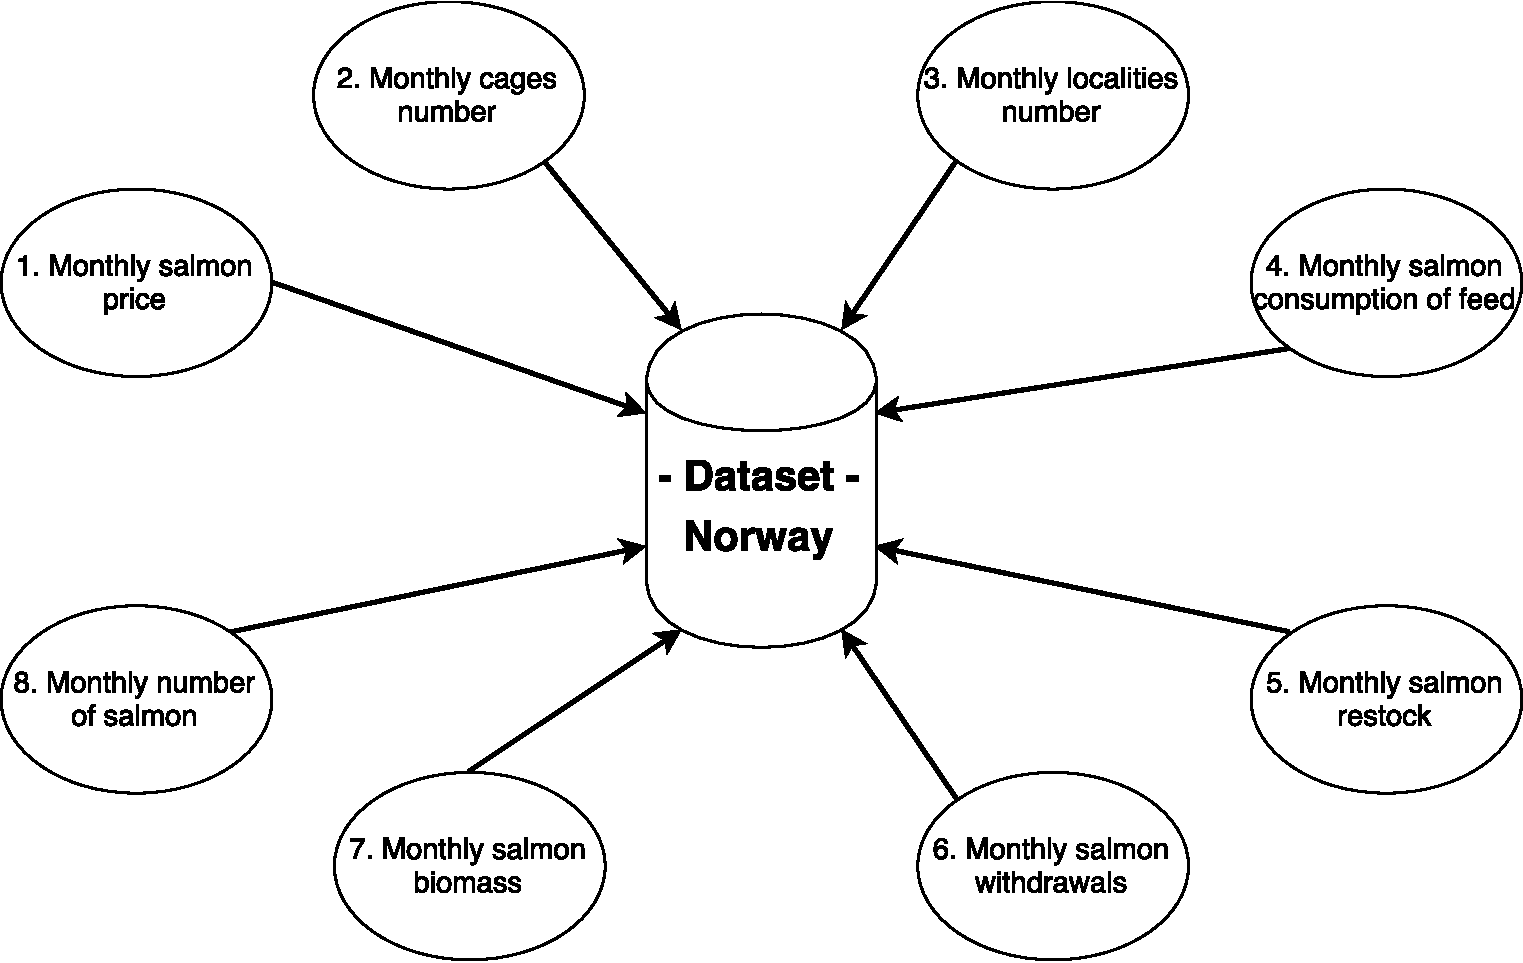
\includegraphics[width=1\textwidth]{Files/Dataset.pdf}}
    \caption{Dataset structure.}
\end{figure}

\begin{table}[ht]
\makebox[\textwidth][c]{
\resizebox{1.2\textwidth}{!}{
    \begin{tabular}{ | l | l | l | l | }
            \hline
\textbf{Input}						& \textbf{Frequency} & \textbf{Period} & \textbf{Location}	\\ \hline
1. Export Salmon Price				& Monthly 			& January 2005 - December 2016 		& Norway 	\\ \hline	
2. Cages							& Monthly 			& January 2005 - December 2016 		& Norway 	\\ \hline									
3. Localities						& Monthly 			& January 2005 - December 2016 		& Norway	\\ \hline
4. Feed consumption					& Monthly 			& January 2005 - December 2016 		& Norway  	\\ \hline
5. Restock							& Monthly 			& January 2005 - December 2016 		& Norway	\\ \hline
6. Withdrawals 						& Monthly 			& January 2005 - December 2016 		& Norway 	\\ \hline
7. Biomass							& Monthly 			& January 2005 - December 2016 		& Norway 	\\ \hline
8. Salmon Number 					& Monthly 			& January 2005 - December 2016 		& Norway	\\ \hline
    \end{tabular}}}
         \caption{Structure of the dataset about Norway.}
    \label{table: Norway_Dataset_struc} 
\end{table}  


\subsection{Dataset about single county} 

\begin{figure}[H]
        \makebox[\textwidth][c]{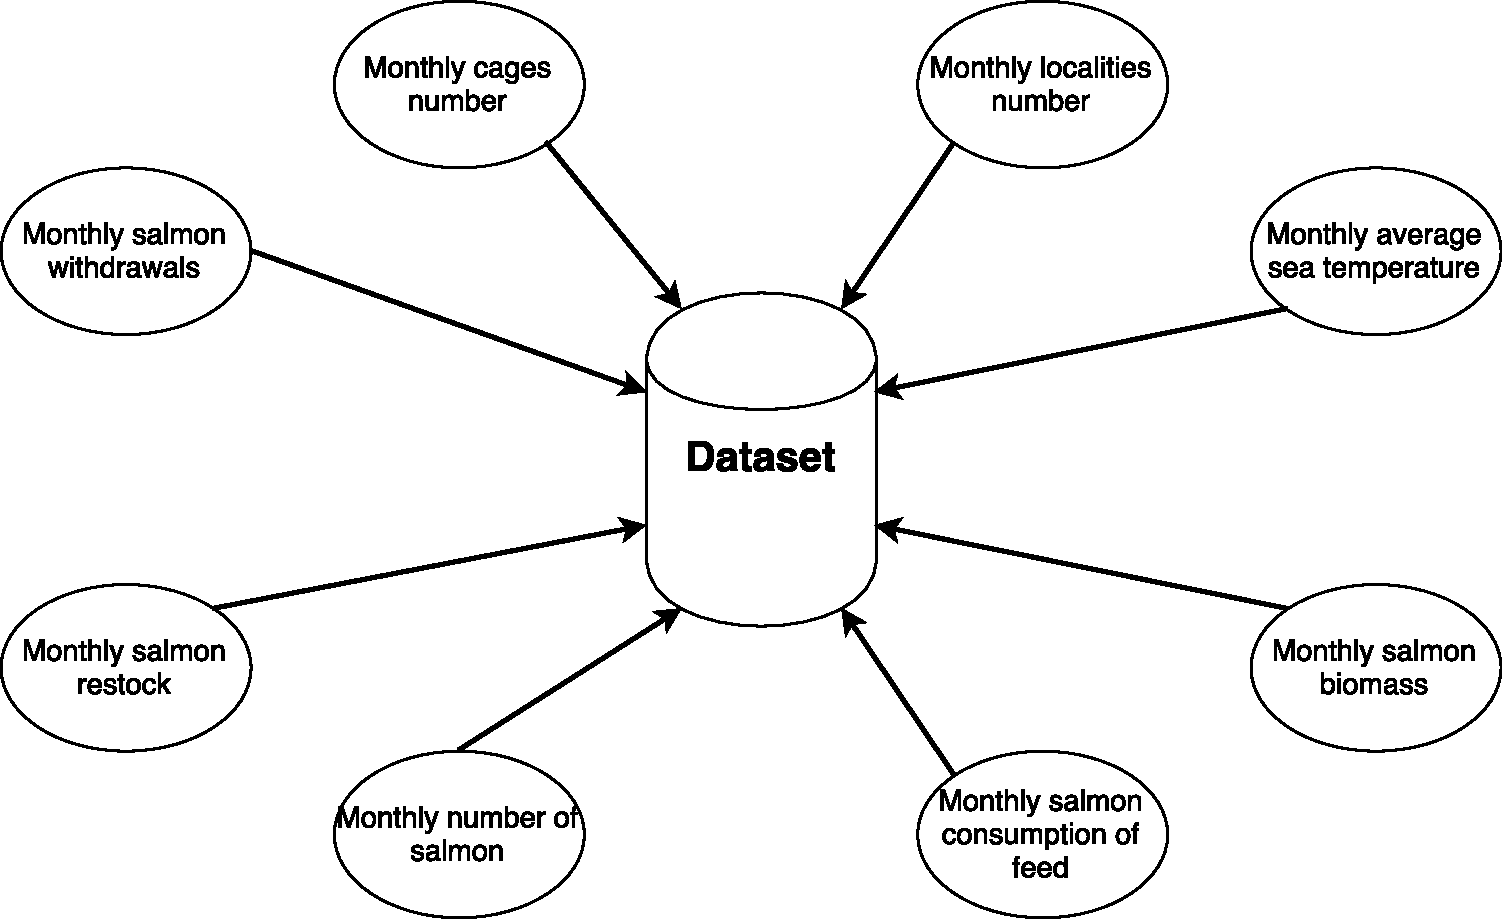
\includegraphics[width=1\textwidth]{Files/Dataset2.pdf}}
    \caption{Dataset structure.}
\end{figure}

\begin{table}[ht]
\makebox[\textwidth][c]{
\resizebox{1.2\textwidth}{!}{
    \begin{tabular}{ | l | l | l | l | }
            \hline
\textbf{Input}						& \textbf{Frequency} & \textbf{Period} & \textbf{Location}	\\ \hline
1. Average Sea Temperature				& Monthly 			& January 2007 - December 2014 		& Single county 	\\ \hline	
2. Cages							& Monthly 			& January 2007 - December 2014 		& Single county 	\\ \hline									
3. Localities						& Monthly 			& January 2007 - December 2014 		& Single county	\\ \hline
4. Feed consumption					& Monthly 			& January 2007 - December 2014 		& Single county  	\\ \hline
5. Restock							& Monthly 			& January 2007 - December 2014 		& Single county	\\ \hline
6. Withdrawals 						& Monthly 			& January 2007 - December 2014 		& Single county 	\\ \hline
7. Biomass							& Monthly 			& January 2007 - December 2014 		& Single county 	\\ \hline
8. Salmon Number 					& Monthly 			& January 2007 - December 2014 		& Single county	\\ \hline
    \end{tabular}}}
         \caption{Structure of the dataset about each norwegian county.}
    \label{table: County_dataset_struc} 
\end{table}      